%!TEX root = ../main.tex
\section{Kritik}
  \subsection*{Unverhältnismäßige geringe Nutzung}
    \begin{frame}<beamer>{Unverhältnismäßige geringe Nutzung}
      \begin{itemize}
        \item
          Abschreckungfaktor ist nicht vorhanden.
        \item
         Umgehungsmöglichkeiten sind auch für Laien möglich.
        \begin{itemize}
          \item TOR-Netzwerk
          \item alternative Emaildienste
          \item bei SMS auf Alternativen umsteigen (zb. Whatsapp)
        \end{itemize}
        \item Durch Vorratsdatenspeicherung hätte weder 9/11 als auch die Attentate in Großbritannien 2005 verhindert werden können
      \end{itemize}
    \end{frame}

\begin{frame}<beamer>{Schwere Strafdaten in Deutschland Statstik}
\begin{itemize}
        \item Schwere Strafdaten in Deutschland Statstik
        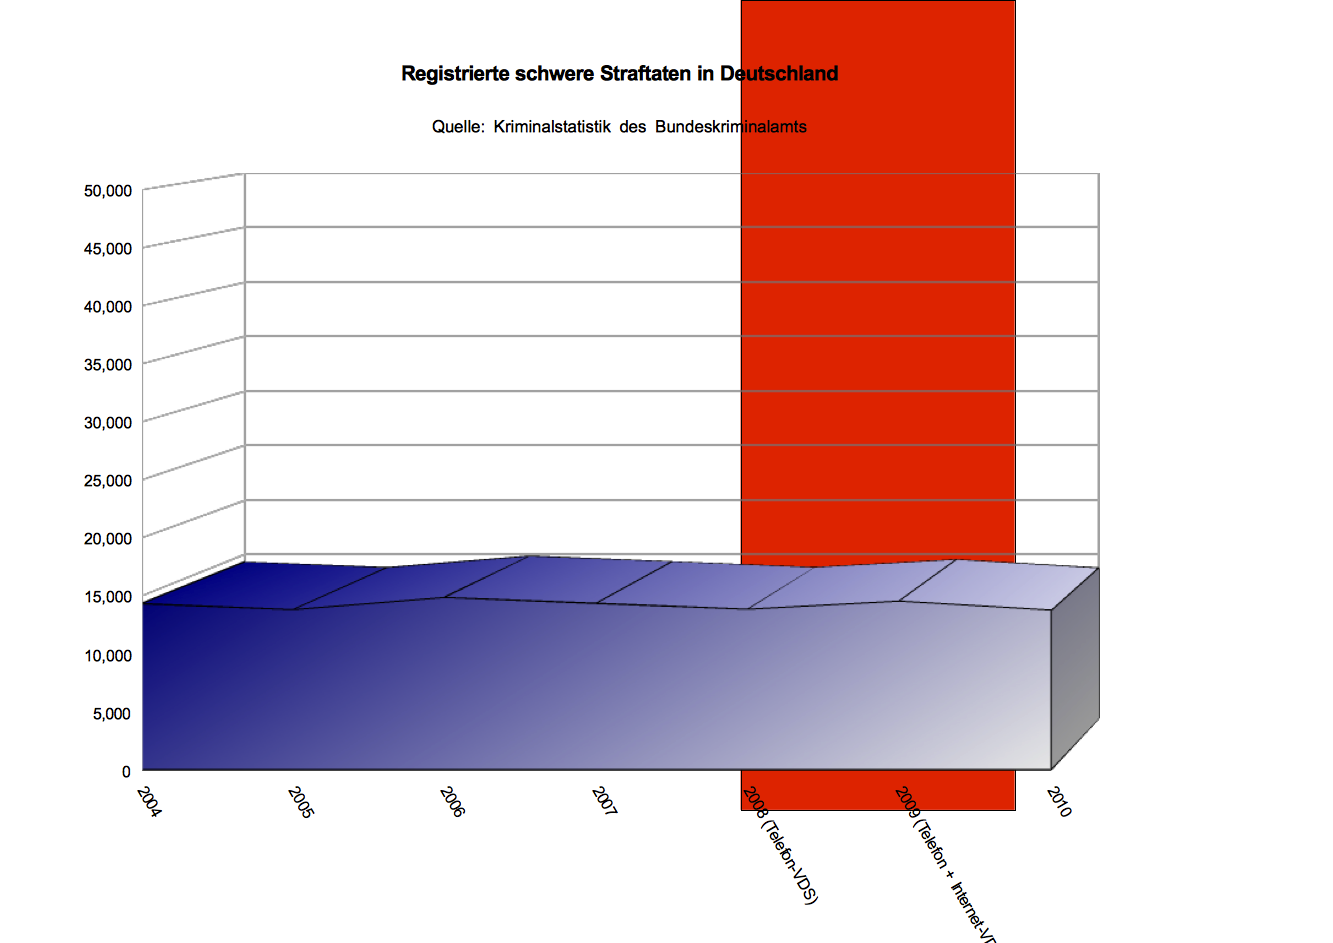
\includegraphics[height=1\textheight]{sections/img/schwere_verbrechen_in_DE.png}
    \end{itemize}
    \end{frame}
    
    \begin{frame}<beamer>{Schwere Verbrechen in Deutschland Aufklärung Statistik}
\begin{itemize}
        \item Schwere Verbrechen in Deutschland Aufklärung Statistik
        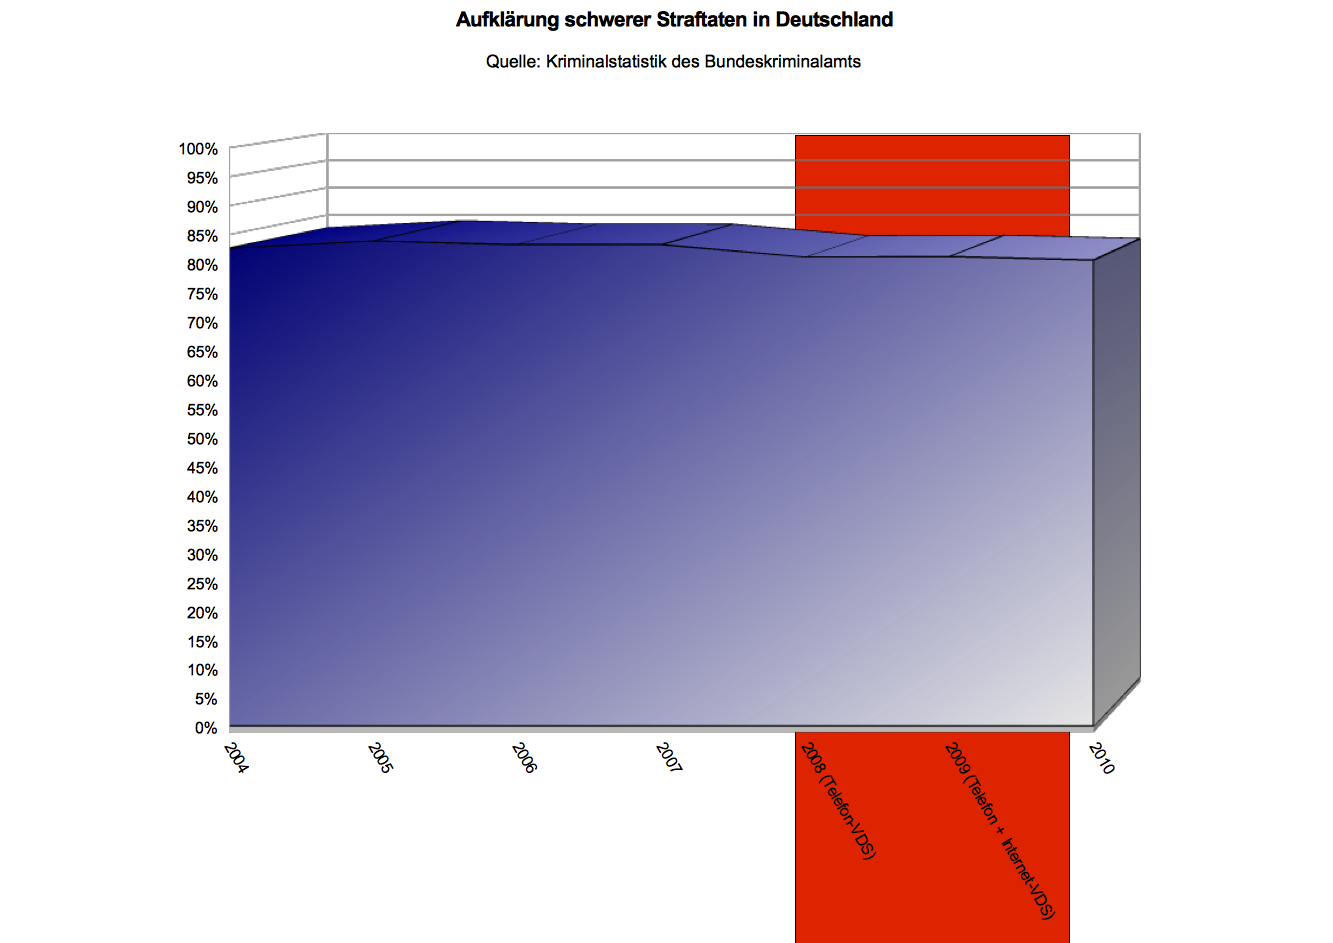
\includegraphics[height=1\textheight]{sections/img/aufklaerung_in_DE.png}
    \end{itemize}
    \end{frame}
      \begin{frame}<beamer>{Internetstrafdaten in Deutschland Statistik}
\begin{itemize}
        \item Internetstrafdaten in Deutschland Statistik
        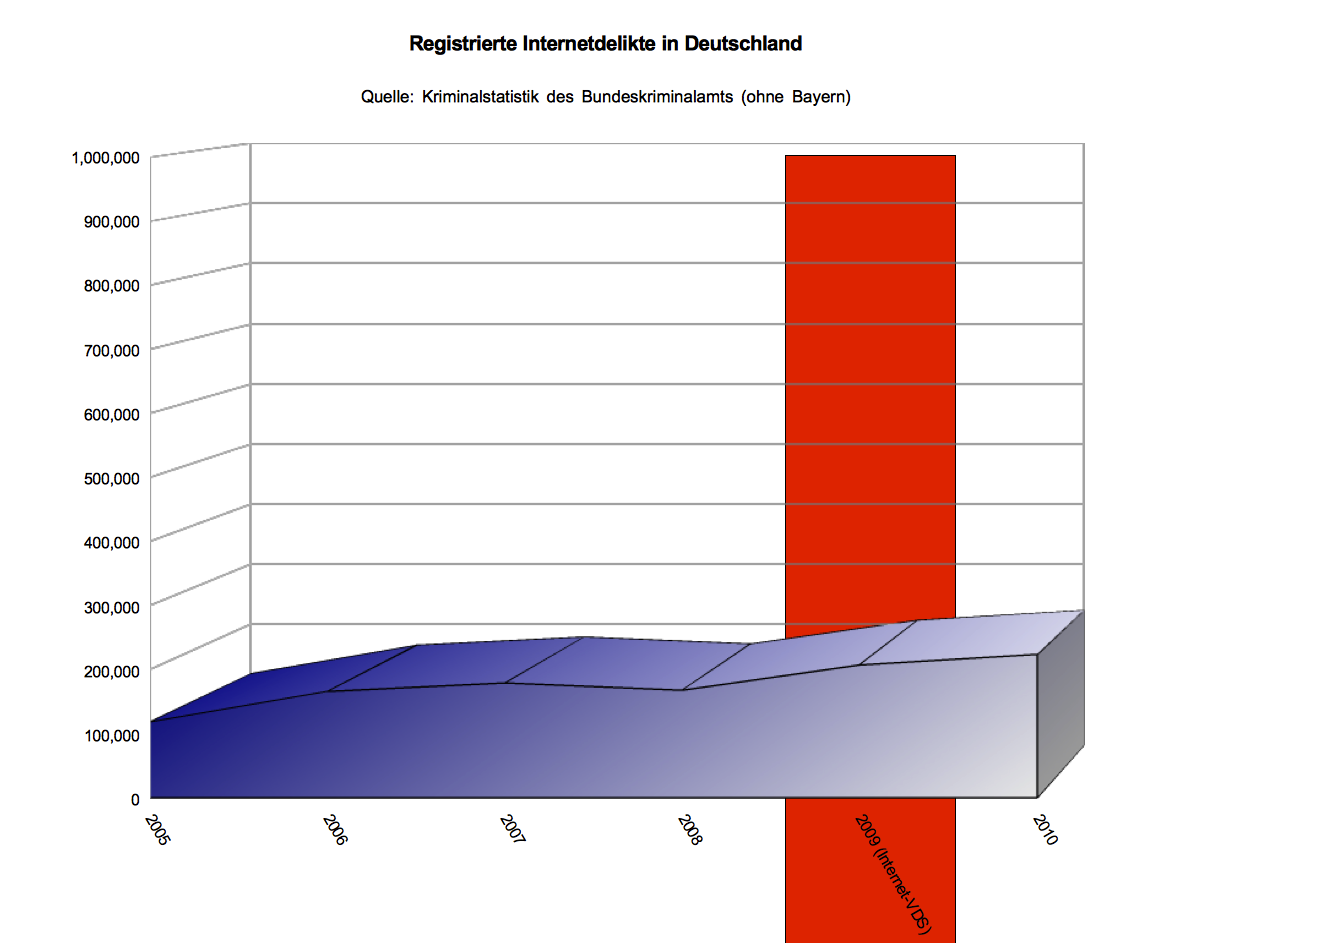
\includegraphics[height=1\textheight]{sections/img/internet_delikte_in_DE.png}
    \end{itemize}
    \end{frame}
          \begin{frame}<beamer>{Internetstrafdaten in Deutschland Aufklärung Statistik}
\begin{itemize}
        \item Internetstrafdaten in Deutschland Aufklärung Statistik
        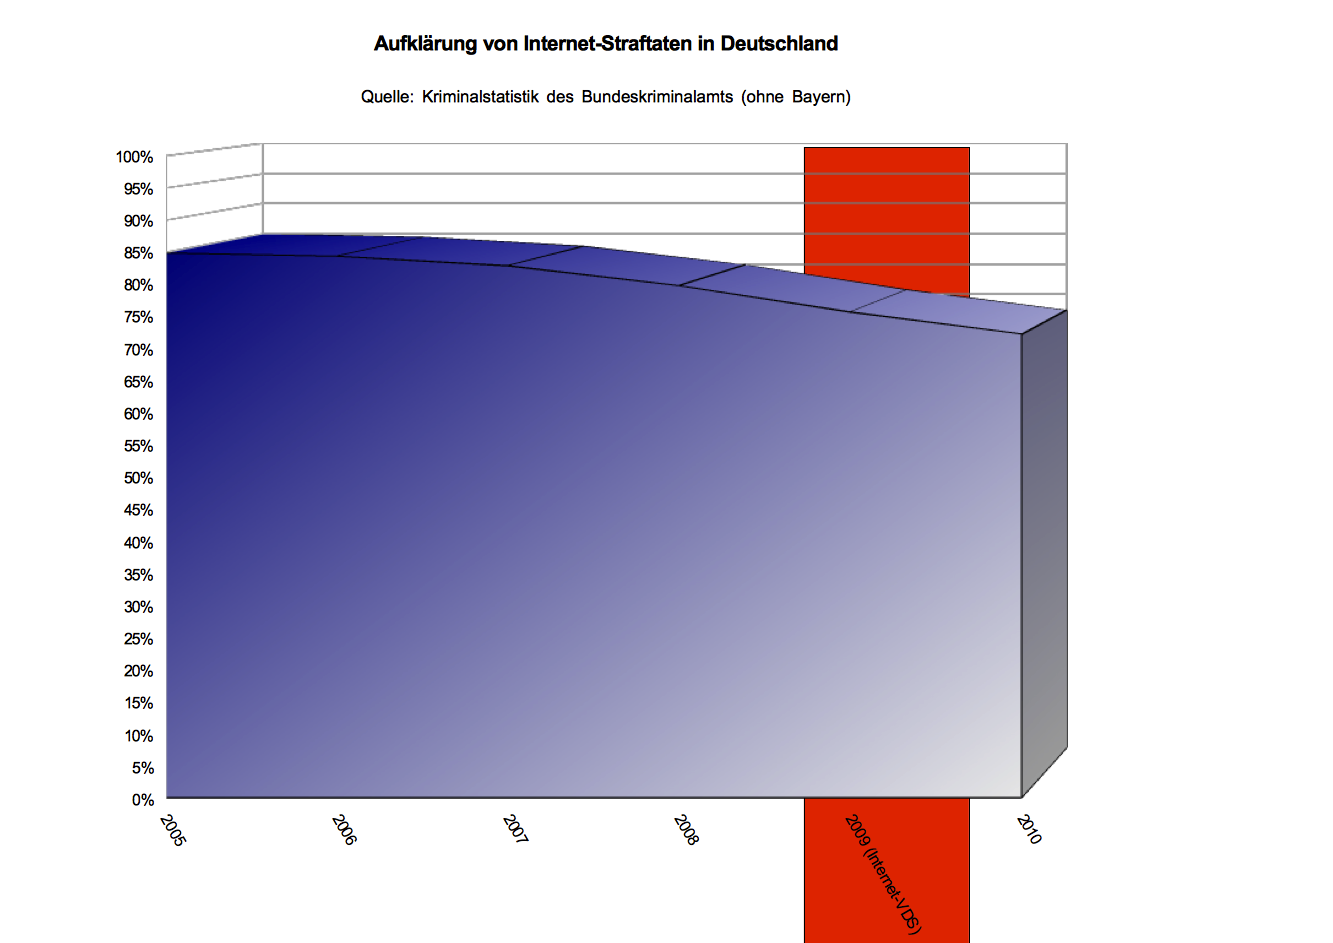
\includegraphics[height=1\textheight]{sections/img/aufklaerung_internetdelikte_DE.png}
    \end{itemize}
    \end{frame}
              \begin{frame}<beamer>{Aufklärungsquote Allgmein}
        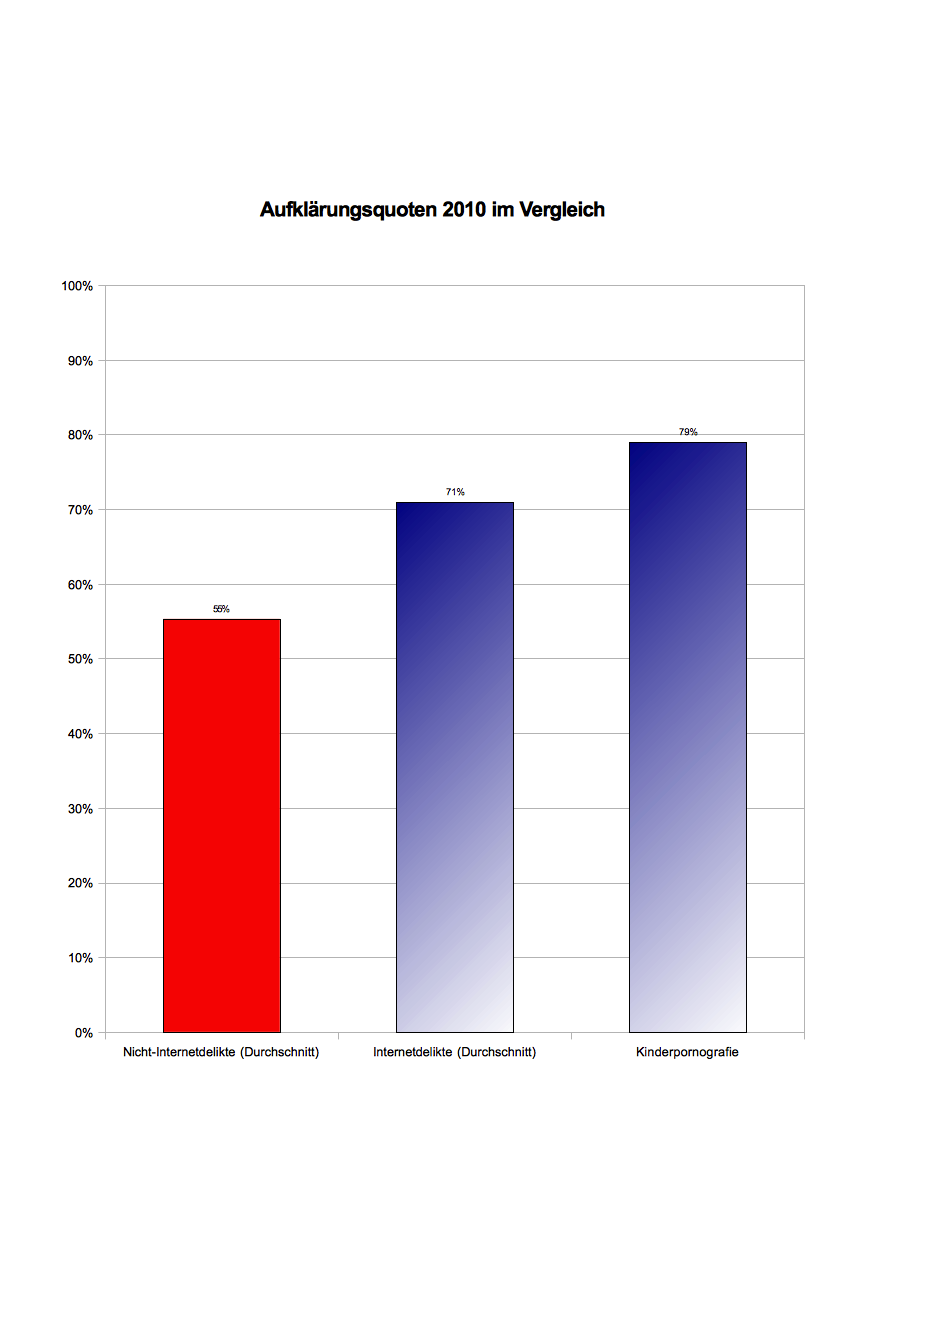
\includegraphics[height=1.25\textheight]{sections/img/aufklaerung.png}
      \end{frame}
              \begin{frame}<beamer>{Interpretation der Statistik des Bundeskriminalamtes}
\begin{itemize}
        \item Die VDS brachte keine Erhöhte Aufklärungsquote
        \item Es konnte keine Senkung der Kriminalitätsrate festgestellt werden
        \item Die Aufklärungsrate der Internetstraftaten sank im Zeitraum der VDS
    \end{itemize}
    \end{frame}
       \begin{frame}<beamer>{Bilanz der Vorratsdatenspeicherung in Österreich}
        \begin{itemize}
        \item 312 Fälle gab es Auskunft über Vorratsdatenspeicherung
        \item 438 Delikte wurde Vorratsdatenspeicherung abgefragt
        \item 161 erledigten Rechtssachen soll in 71 Fällen die Vorratsdatenspeicherung eine Betrag zur Aufklärung geleistet haben
        \item die meisten Abfragen gab es nicht bei schweren Verbrechen, wie Terrorismus und Mord sondern
        \item die meisten gab es bei Diebstahl(106) und Stalking
        \item Kosten für die Steuerzahler bisher 2,3 Millionen Euro
        \item Man rechnet mit jährliche Gesamtkosten von 8 Millionen Euro.
        \item Stand: 09.07.2013 
         \end{itemize}
    \end{frame}
    \begin{frame}<beamer>{Straftaten in Osterreich Vergleich}
      \begin{quote}
        Dennoch zeigten die Daten der österreichischen Vorratsdatenspeicherung, daß die angeblich schwersten Straftaten, bei denen die Datensätze abgerufen werden sollten, in Wahrheit in erster Linie Diebstahlsdelikte waren, außerdem Stalking. Bei Organisierter Kriminalität oder Taten, die als Terror definiert sind, wurden die zwangsweise gespeicherten Daten in genau null Fällen verwendet.

        \attrib{Chaos Computer Club}
      \end{quote}
    \end{frame}



  \subsection*{Missbrauch und Irrtumsrisiko}
    \begin{frame}<beamer>{Missbrauch und Irrtumsrisiko}
      \begin{itemize}
        \item
          Telekommunikationsdaten haben eine sehr hohe Aussagekraft
      \begin{itemize}
         \item mit Methoden von Data-mining können scheinbar belanglose Daten eine hohe Aussagekraft bekommen
      \end{itemize}
        \item
          Rückschlüsse auf die gesamte Lebensituation möglich
 \item viele Interessensgruppen haben Interesse an den sensiblen Daten
          \begin{itemize}
         \item Behörden/Staat
         \item politische Gruppierungen
         \item Personen aus Privatenumfeld
      \end{itemize}
 
      \end{itemize}
    \end{frame}

  \subsection*{Juristische Argumente}
    \begin{frame}<beamer>{Juristische Argumente}
      \textbf{Verstoß gegen Europarecht}
      \begin{quote}
        Der Gerichtshof sieht in der Verpflichtung zur Vorratsspeicherung dieser Daten und der Gestattung des Zugangs der zuständigen nationalen Behörden zu ihnen einen besonders schwerwiegenden Eingriff der Richtlinie in die Grundrechte auf Achtung des Privatlebens und auf Schutz personenbezogener Daten.

        \attrib{Gerichtshof der Europäischen Union}
      \end{quote}
    \end{frame}

    \begin{frame}<beamer>{Juristische Argumente}
      \textbf{Verstoß gegen deutsches Recht}
      \begin{quote}
        Eine sechsmonatige, vorsorglich anlasslose Speicherung von Telekommunikationsverkehrsdaten durch private Diensteanbieter, wie sie die Richtlinie 2006/24/EG des Europäischen Parlaments und des Rates vom 15. März 2006 (ABl L 105 vom 13. April 2006, S. 54; im Folgenden: Richtlinie 2006/24/EG) vorsieht, ist mit Art. 10 GG nicht schlechthin unvereinbar; auf einen etwaigen Vorrang dieser Richtlinie kommt es daher nicht an.

        \attrib{Bundesverfassungsgericht}
      \end{quote}
    \end{frame}

    \begin{frame}<beamer>{Juristische Argumente}
      \textbf{Versto"s gegen die Europ"aische Menschenrechtskonvention}
      \begin{quote}
        Die Erfassung aller Verbindungsdaten könne \"nicht als vereinbar mit den Bestimmungen der Verfassung und der Europäischen Menschenrechtskonvention erachtet werden\".

        \attrib{AK-Vorratsdatenspeicherung}
      \end{quote}
    \end{frame}

    \subsection*{Demonstrationen}
    \begin{frame}<beamer>{Protestbewegungen}
      \begin{figure}
        \begin{subfigure}[b]{0.5\textwidth}
          \begin{itemize}
            \item Arbeitskreis Vorratsdatenspeicherung
            \item Unterst"utzung aus unterschiedlichsten Bereichen z.B.:
              \begin{itemize}
                \item CCC
                \item Deutsche Journalistinnen- und Journalisten-Union
                \item Internationale Liga für Menschenrechte
                \item Deutscher Anwaltverein
              \end{itemize}
            \item 11. Oktober 2008: Demonstration {\em Freiheit statt Angst} mit 15.000 Teilnehmern in Berlin
          \end{itemize}
        \end{subfigure}
        \begin{subfigure}[b]{0.3\textwidth}
          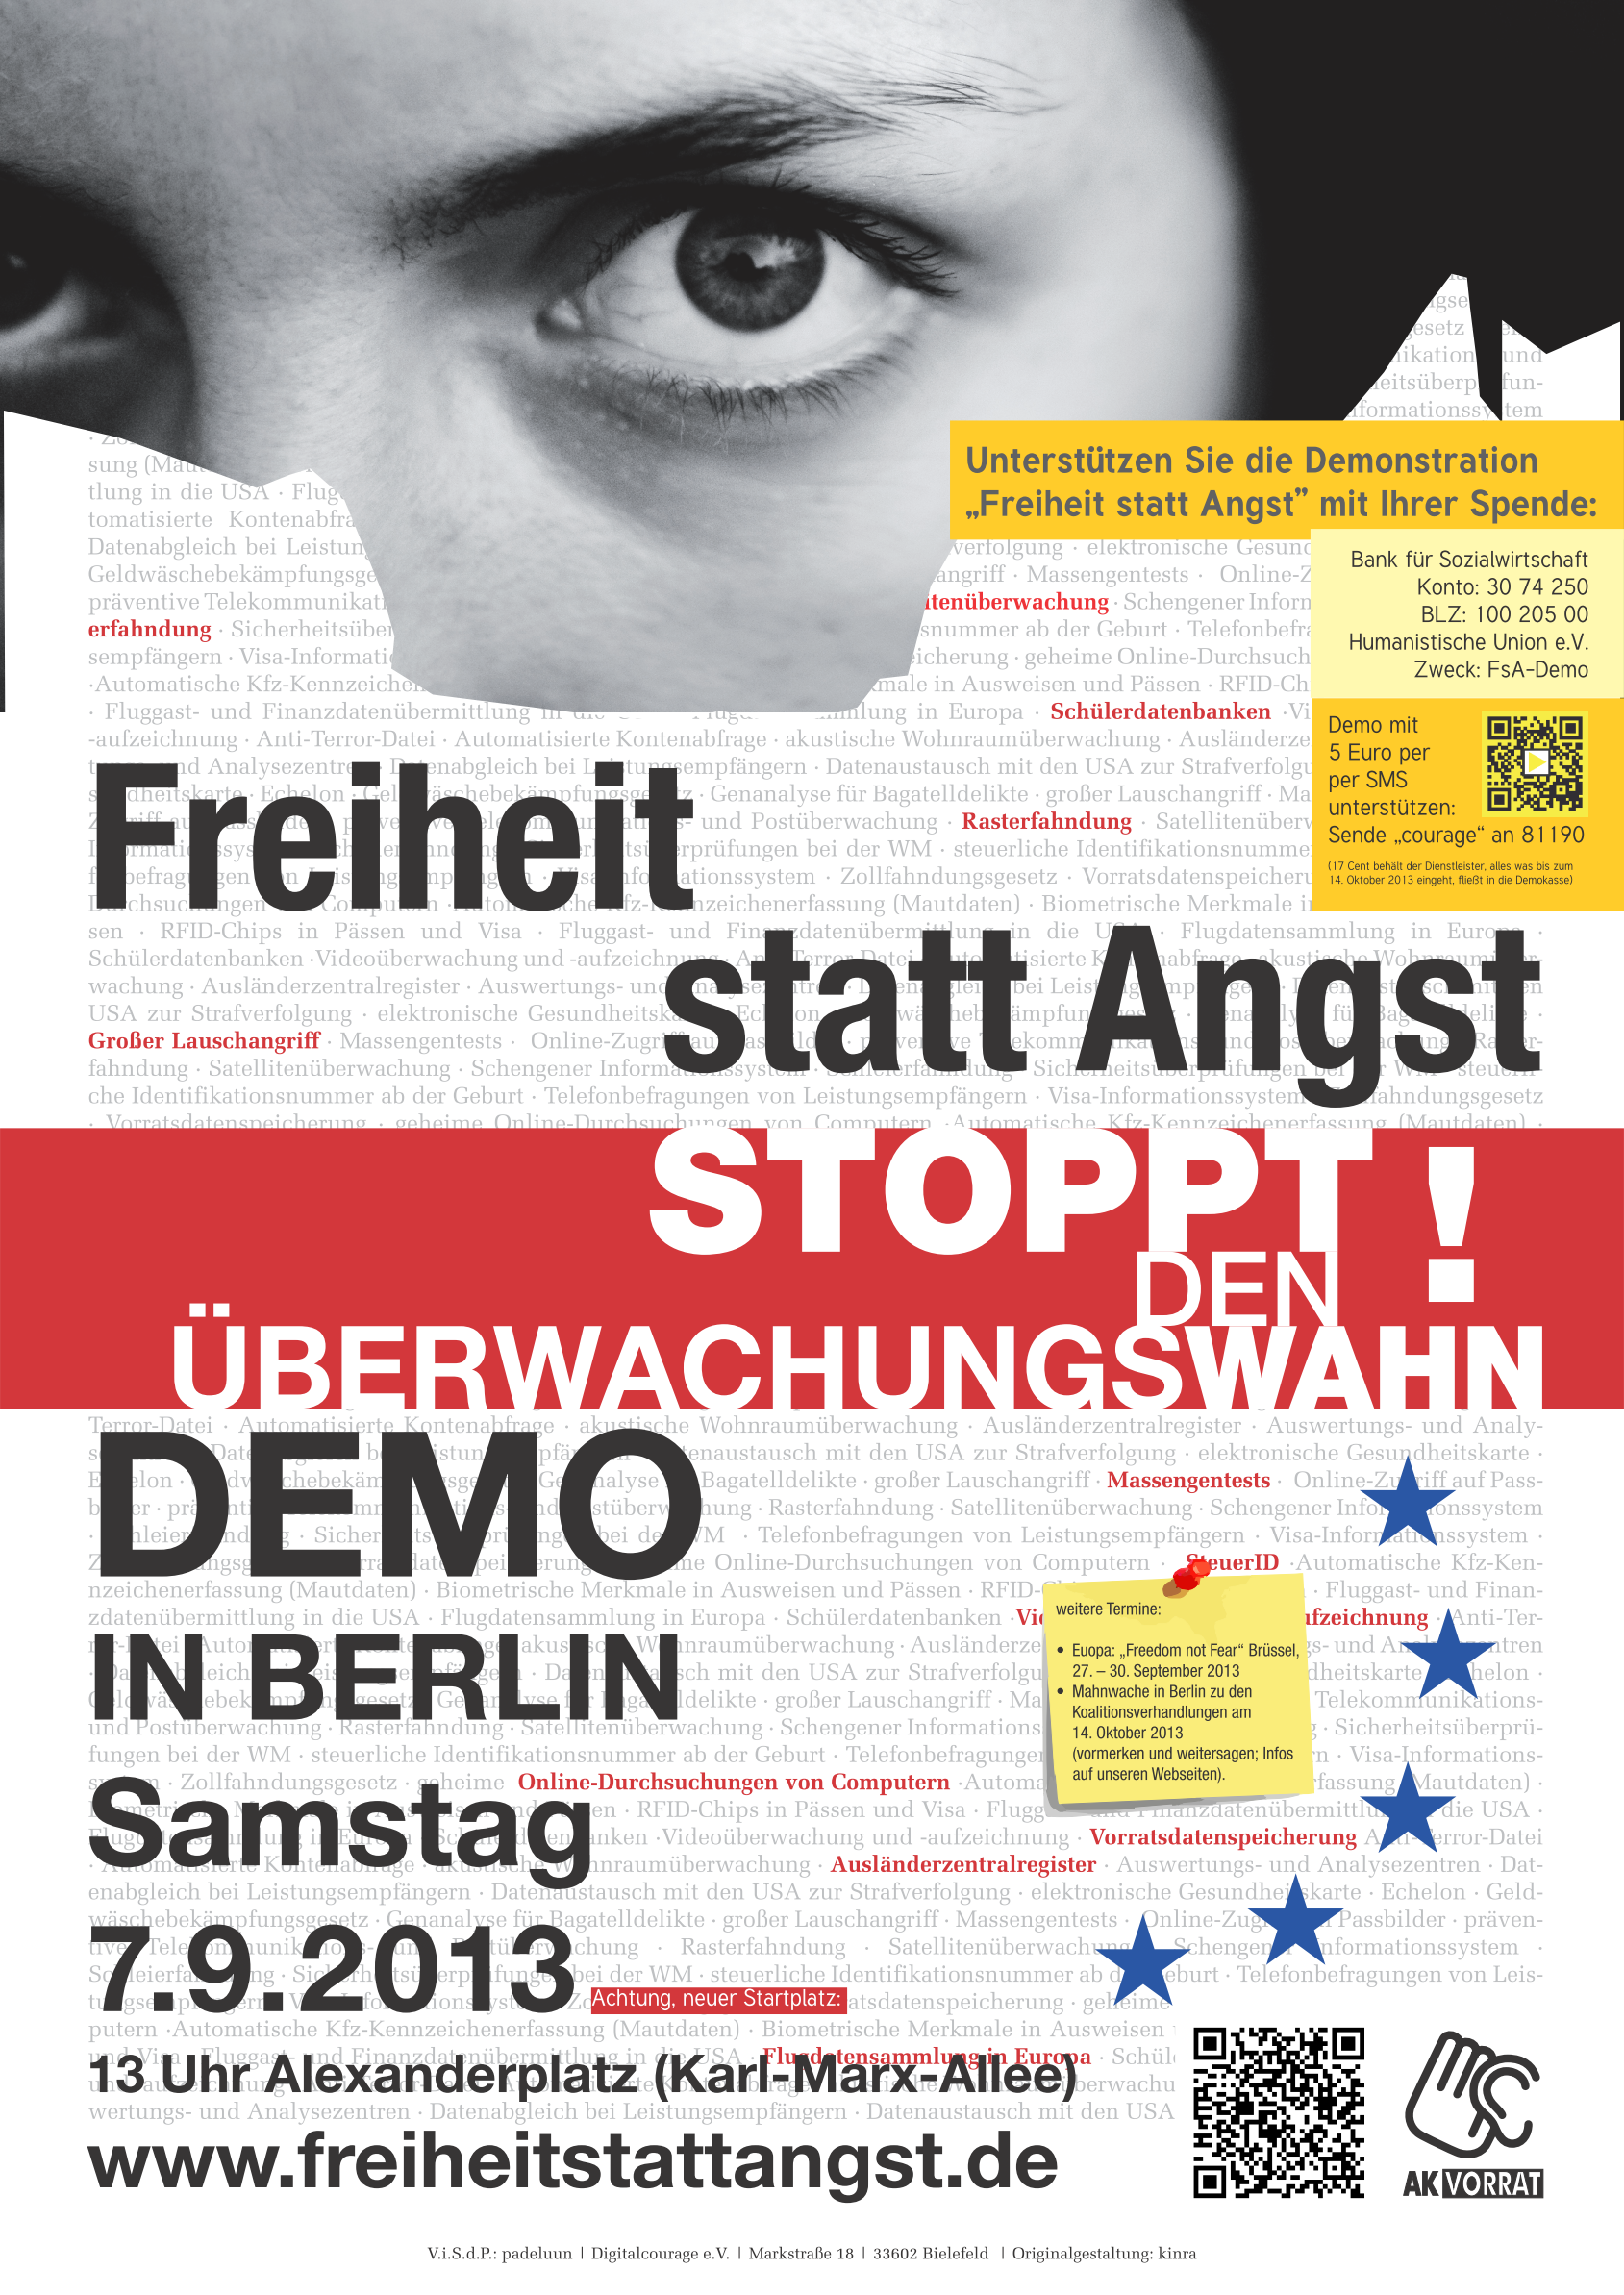
\includegraphics[scale=0.05]{sections/img/freiheit_statt_angst.png}
          \caption{Freiheit statt Angst}
          \label{fig:freiheit}
        \end{subfigure}
      \end{figure}
    \end{frame}

    \begin{frame}<beamer>{Kritik aus dem historischen Kontext}
       \begin{itemize}
        \item totalitäre Überwachung im 3. Reich
        \item Überwachung der Stasi in der DDR
        \item Befürchtung die Ausweitung der Überwachung könnte die Demokratie aushöhlen und letztlich abschaffen.
      \end{itemize}
    \end{frame}

